
Da davon ausgegangen wird, dass der User sich nicht nach jeder Nutzung ab- und wieder anmeldet, erscheint im alltäglichen Gebrauch der in Abbildung \ref{fig:homescreen_alle} dargestellte Bildschirm zuerst. Demnach bietet es sich an Ereignisse wie neue Matches und neue Nachrichten hier anzuzeigen. Diese werden wie Abbildungen \ref{fig:homescreen_a} und \ref{fig:homescreen_b} zeigen klar strukturiert in Abschnitte eingegliedert, welche mit Überschriften kenntlich gemacht sind. Die einzelnen Matches befinden sich mit allen dazugehörenden Funktionen und Informationen jeweils auf einer Karte. Durch diese Karten kann mit einer von anderen \mbox{Apps} bekannten horizontalen Swipemechanik navigiert werden. Weiterführende Funktionen wie das Starten eines Chats oder das Löschen des Matches werden durch  Antippen von allgemein verständlichen Icons ausgeführt. \\
Auch auf diesem Screen findet sich einerseits das bereits eingeführte Farbschema wieder und es werden andererseits ebenfalls Semantiken verwendet. Bei den neuen Nachrichten wird jeweils der Benutzername vorgelesen und bei den neuen Matches je nach ausgewähltem Bereich der Filmname, die Icons oder der Text dazwischen.\\
Am unteren Bildschirmrand ist eine sogenannte Bottom-Navigation-Bar zu sehen. Sie ermöglicht eine kompakte und anschauliche Navigation durch die relevanten Bildschirme. Außerdem zeigt sie an welcher Bildschirm aktuell ausgewählt ist, wobei diese Information wie in Abschnitt \ref{sec:bf-streamswipe} erarbeitet nicht ausschließlich auf einer Farbänderung basieren sollte und deshalb das ausgewählte Icon durch Hinzufügen von Text hervorgehoben wird. Liest der Screenreader die Semantik hiervon, gibt er die Bezeichnung des aktuellen Bildschirms sowie die Anzahl der weiteren Möglichkeiten an. \\
%TODO Motorische Herausforderungen!!! Anklicken des Filmposters aktiviert auch Chat?

\begin{figure}[H]
	\begin{subfigure}{0.33\textwidth}
	\centering
	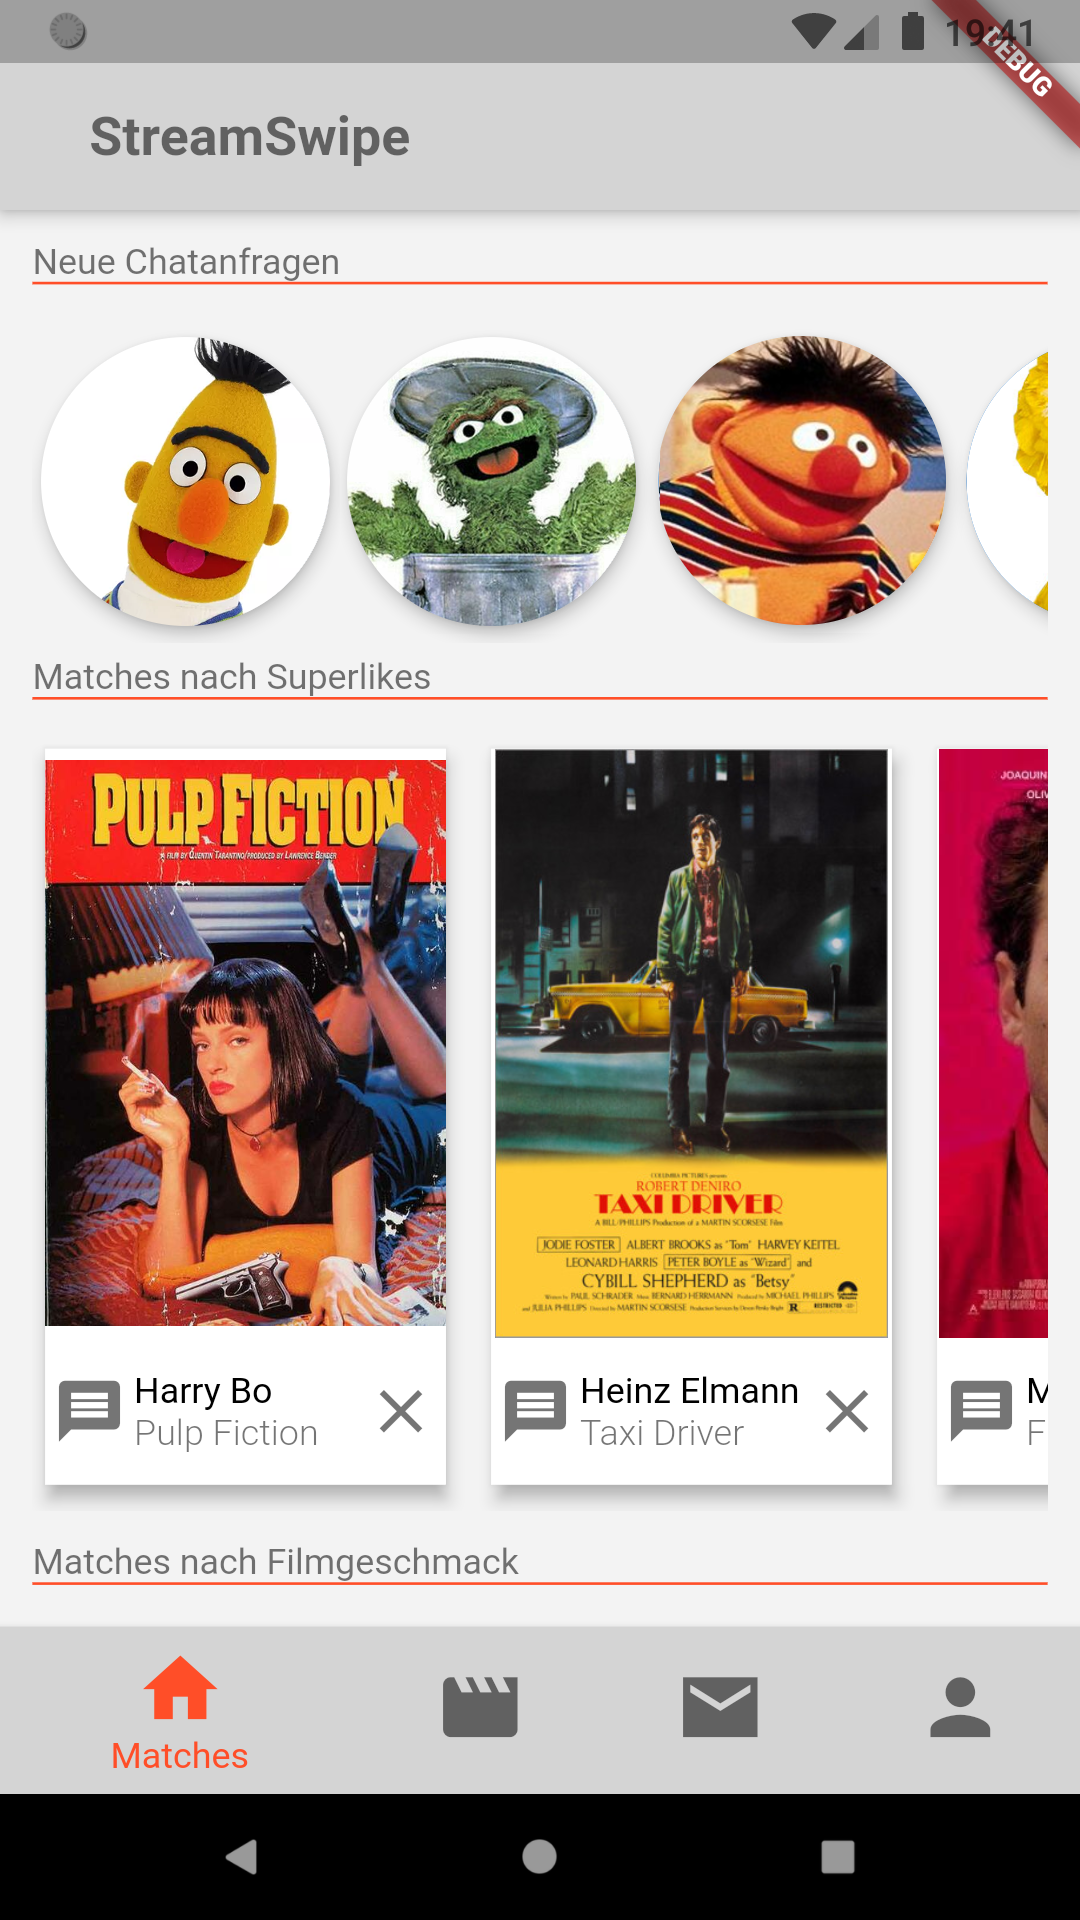
\includegraphics[scale=0.13]{Benutzeroberfläche/images/screenshot_homescreen_1.png}
	\caption{}
	\label{fig:homescreen_a}
	\end{subfigure}
	\begin{subfigure}{0.33\textwidth}
	\centering
	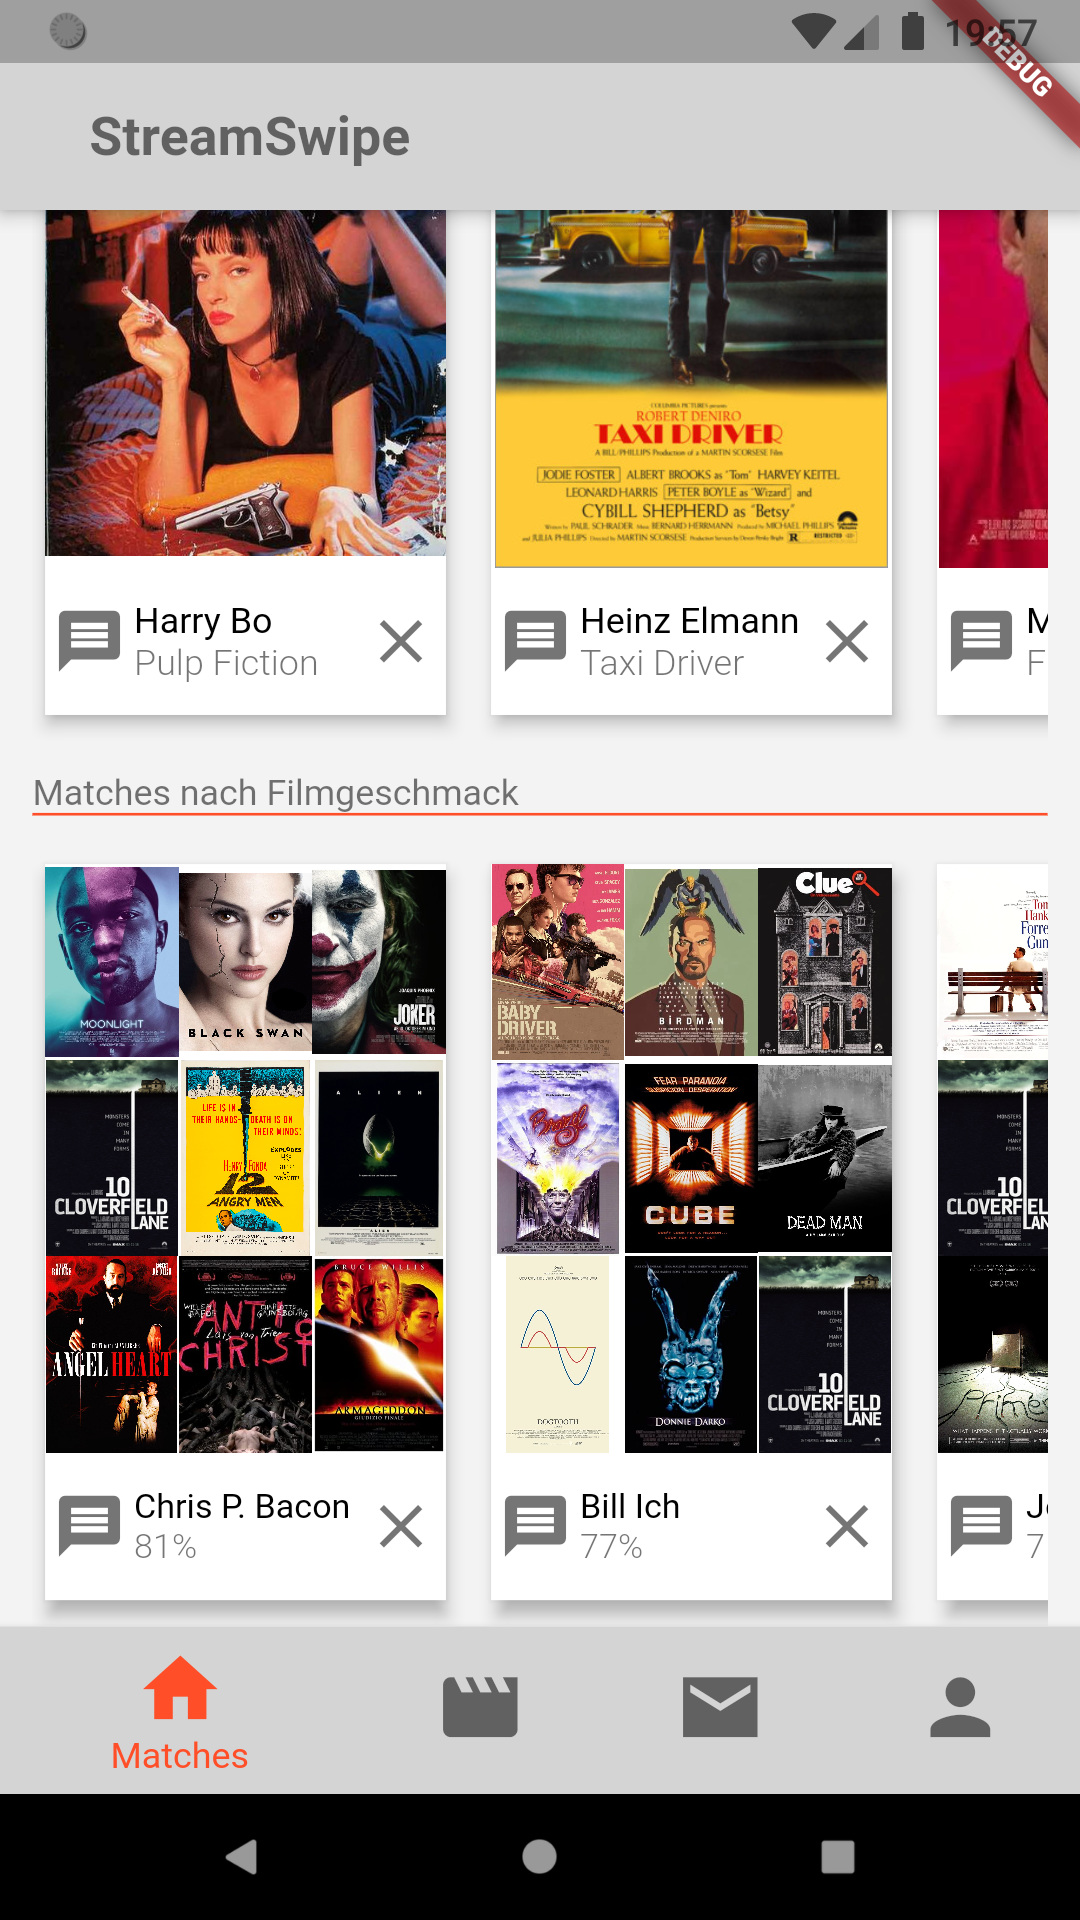
\includegraphics[scale=0.13]{Benutzeroberfläche/images/screenshot_homescreen_2.png}
	\caption{}
	\label{fig:homescreen_b}
	\end{subfigure}
	\begin{subfigure}{0.33\textwidth}
	\centering
	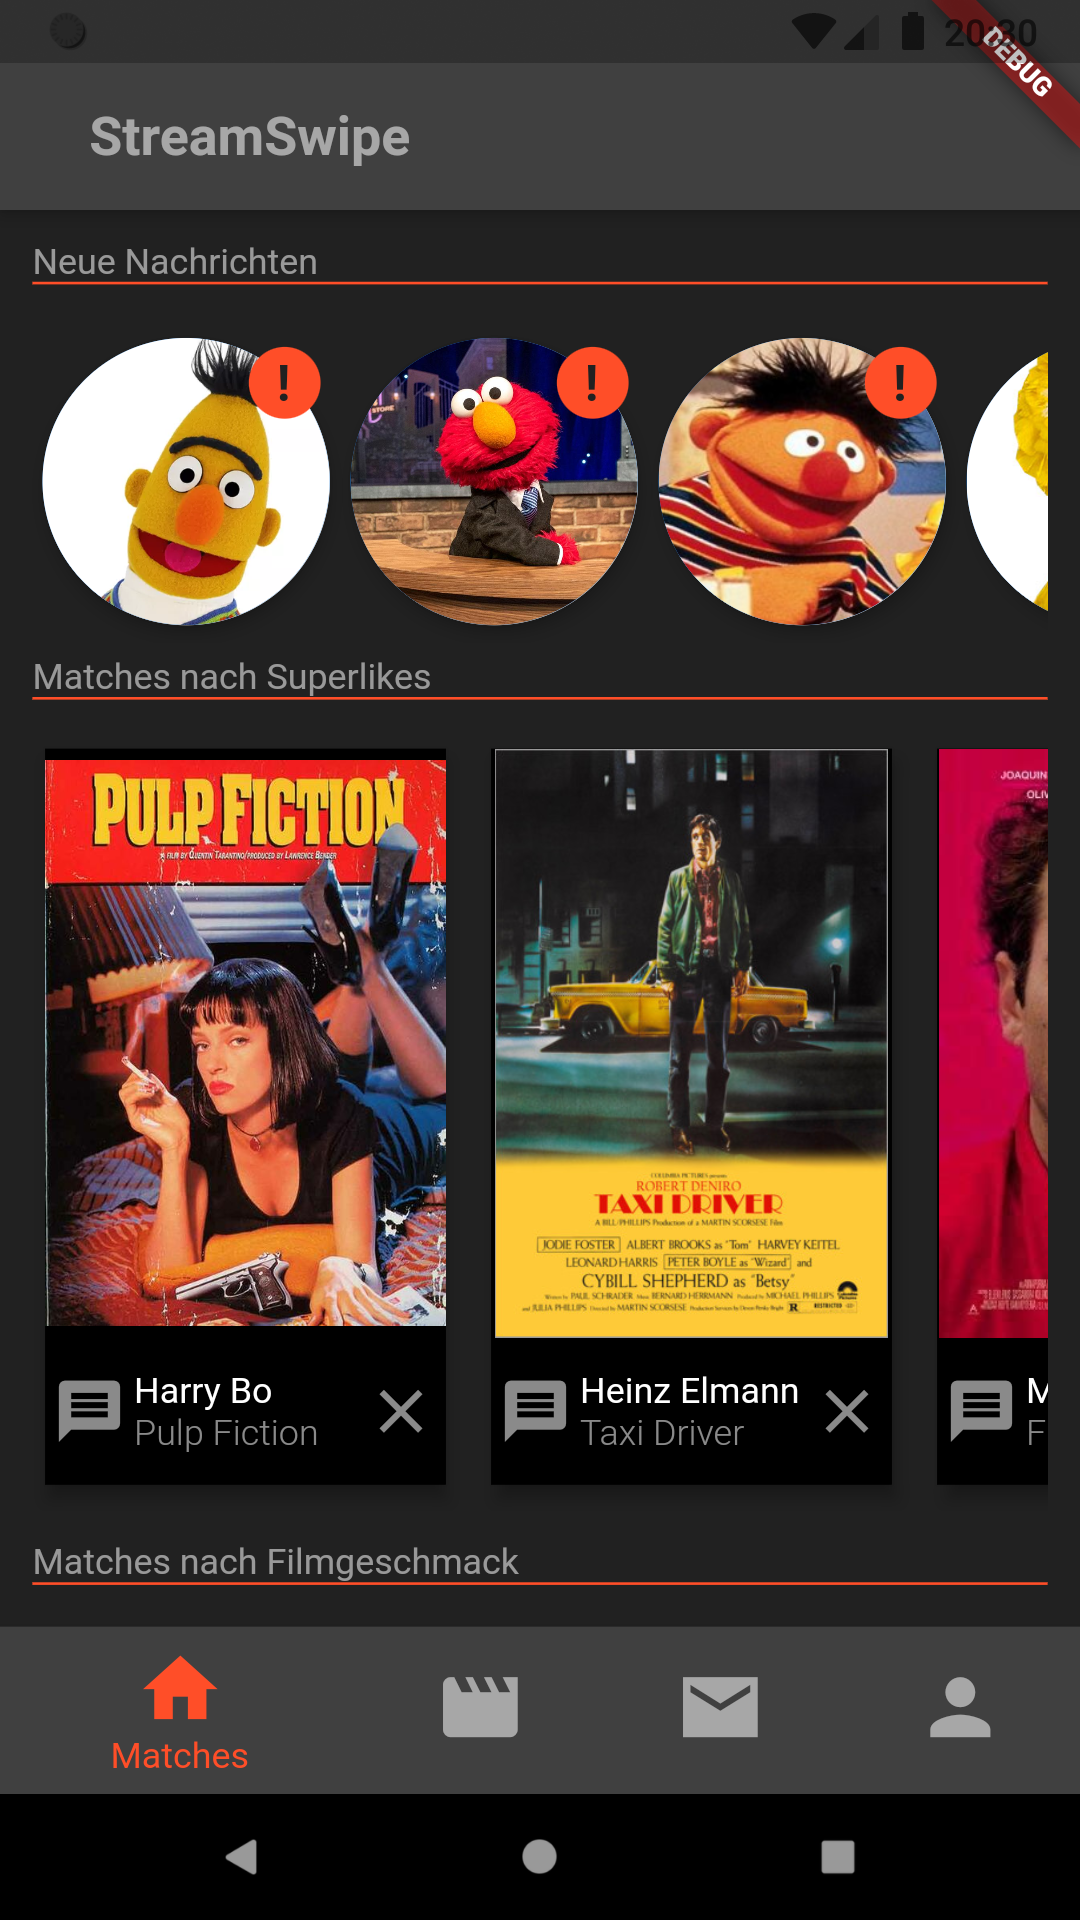
\includegraphics[scale=0.13]{Benutzeroberfläche/images/screenshot_darkmode_1.png}
	\caption{}
	\label{fig:homescreen_c}
	\end{subfigure}
\caption[Screenshots des Home-Screens]{Der Home-Screen, der beim Öffnen der App zuerst gezeigt wird und Neuigkeiten wie neue Nachrichten und Matches zusammenfasst. Um den gesamten Inhalt dieser Seite sehen zu können, wird in (a) der obere Abschnitt und in (b) der untere Abschnitt gezeigt. Hat der User in den Systemeinstellungen den dunklen Modus aktiviert, so wird (c) der Home-Screen wie alle anderen Screens angepasst.}
\label{fig:homescreen_alle}
\end{figure}

